%%% Sekce – Vyřízení a potvrzení objednávky
%%%%% Wording: ✅
%%%%% Styling: ✅
%%%%% References: ✅
%%% --------------------------------------------------------------
\section{Vyřízení a potvrzení objednávky}
\label{sec:implementace-checkout}
Proces vyřízení objednávky je posledním hlavním krokem nákupu vstupenek, který je touto prací řešen.
Je implementován jako jednoduchý formulář, který je zobrazen uživateli po naplnění košíku vstupenkami.
Tento formulář a jeho správa je opět pouze dalším rozšířením logiky košíku.
S pomocí hooku \texttt{useForm} z knihovny React Hook Form je implementována logika formuláře pomocí pouze několika málo řádků kódu.
Formulář se skládá z několika polí reprezentovaných validačním schématem pomocí knihovny Zod v ukázce~\ref{lst:checkout-contact-details-schema}.

\begin{listing}[h]
    \begin{minted}{typescript}
/**
 * Cart contact details validation schema
 * @export
 */
export const useCartContactDetailsSchema = z.object({
	firstName: z.string().nonempty(),
	lastName: z.string().nonempty(),
	email: z.string().email(),
	phone: z.string().nonempty(),
	message: z.string().optional(),
	acceptTerms: z.boolean().refine((v) => v === true, { message: 'You must accept terms and conditions' }),
});
    \end{minted}
    \caption{Validační schéma kontaktních údajů formuláře}
    \label{lst:checkout-contact-details-schema}
\end{listing}

Formulářová políčka jsou poté vykreslena s pomocí knihovny Mantine, která kromě mnoha dalších komponent poskytuje komponentu \texttt{TextInput}, která je primárně použita pro ovládání těchto polí.
Jelikož se jedná o komponentu z knihovny třetí strany, je pomocí komponenty \texttt{Controller} z knihovny \texttt{react-hook-form} připojena k formuláři, která řeší správu stavu formuláře.
V ukázce kódu~\ref{lst:controlled-text-input} je zobrazeno připojení komponenty \texttt{TextInput} k poli \texttt{firstName} ve formuláři.

\begin{listing}[h]
    \begin{minted}{typescript}
<Controller<CartTypes.ContactDetails, 'firstName'>
	name="firstName"
	control={cart.contactForm.control}
	render={({ field, fieldState }) => (
		<TextInput label="First name" description="Enter your first name" {...field} error={fieldState.error?.message} />
	)}
/>
    \end{minted}
    \caption{Ukázka kontrolované komponenty \texttt{TextInput}}
    \label{lst:controlled-text-input}
\end{listing}

Ostatní formulářové prvky jsou poté vykresleny obdobným způsobem.

%%% Podsekce – Metoda platby
%%%%% Wording: ✅
%%%%% Styling: ✅
%%%%% References: ✅
%%% --------------------------------------------------------------
\begin{subsection}{Metoda platby}
    \label{subsec:implementace-checkout-payment-method}
    Kromě kontaktních údajů formulář obsahuje také výběr platební metody.
    I když samotný proces platby není součástí této práce, obsahuje formulář jednoduchý výběr platebních metod.
    Tyto metody jsou zobrazeny jako jednoduchá skupina radio tlačítek za pomoci komponenty \texttt{RadioGroup} z knihovny Mantine.
    Na ukázce kódu~\ref{lst:checkout-payment-method} je zobrazen jednoduchý číselník podporovaných platebních metod.

    \begin{listing}[h]
        \begin{minted}{typescript}
/**
* PaymentMethod enumeration
* @export
*/
export enum PAYMENT_METHOD {
	CREDIT_DEBIT_CARD = 'CREDIT_DEBIT_CARD',
	APPLE_PAY = 'APPLE_PAY',
	PAYPAL = 'PAYPAL',
}
        \end{minted}
        \caption{Číselník podporovaných platebních metod}
        \label{lst:checkout-payment-method}
    \end{listing}

    Výběr podporovaných platebních metod byl zvolen na základě metod navržených v sekci~\ref{subsec:narvh-ui-transformace-uzivatelskych-pribehu-vyrideni-a-potvrzeni-objednavky}.
    V reálném světě by byly metody platby implementovány například na základě integrace platební brány.

    Jako mikro rozšíření obsahuje košík jednoduchý stav aktuálně vybrané platební metody, který by byl dále použit v procesu platby.
\end{subsection}

%%% Podesekce – Souhrn objednávky
%%%%% Wording: ✅
%%%%% Styling: ✅
%%%%% References: ✅
%%% --------------------------------------------------------------
\begin{subsection}{Souhrn objednávky}
    \label{subsec:implementace-checkout-souhrn}
    Jako požadavek na uživatelské rozhraní bylo stanoveno, že stránka dokončení objednávky musí obsahovat její souhrn.
    Tento souhrn je zobrazen jako karta obsahující seznam všech vstupenek v košíku.
    Mimo jiné slouží také jako místo pro tlačítko k dokončení objednávky, které je podmíněno platností formuláře, které zahrnuje především akceptaci obchodních podmínek.
    Po kliknutí na tlačítko je formulář validován oproti validačnímu schématu zobrazenému v ukázce kódu~\ref{lst:checkout-contact-details-schema}.
    Pokud validací projde, je zavolán handler \texttt{createOrderHandler()} řešící vytvoření objednávky, který simuluje volání \ac{api} a poté uživatele přesměruje na stránku s potvrzením objednávky.
    Jeho implementace je zobrazena v ukázce kódu~\ref{lst:create-order-handler}.

    \begin{listing}[H]
        \begin{minted}{typescript}
/** create order handler */
const createOrderHandler = useHandler<Types.UseCart.CreateOrderCb>(
	async (contactDetails) => {
		console.log('[Cart] Creating order...');
		multiViewProvider.changeView(Types.TMultiView.ORDER_RESULT);
		await simulatedNetworkDelay('heavy');
		_setReservation(null);
		_setCartedTickets([]);
		return {
			orderId: uuidv4(),
			orderNumber: randomIntBetween(100000, 999999).toString(),
			status: 'Paid',
			created: subSeconds(new Date(), 64),
			paid: new Date(),
			paymentMethod,
			amount: cartTotal,
			tickets: cartedTickets,
		};
	},
	{
		deps: [cartedTickets, paymentMethod, cartTotal],
	},
);
        \end{minted}
        \caption{Implementace handleru pro vytvoření objednávky}
        \label{lst:create-order-handler}
    \end{listing}

    Jak je uvedeno v ukázce kódu~\ref{lst:create-order-handler}, tento handler vytvoří falešnou novou objednávku za účelem jejího pozdějšího zobrazení na stránce s potvrzením.
    Souhrn objednávky spolu s již popsanými kontaktními údaji a formulářem pro výběr platební metody je zobrazeno na obrázku~\ref{fig:seating-map-checkout}.

    \begin{figure}[H]
        \centering
        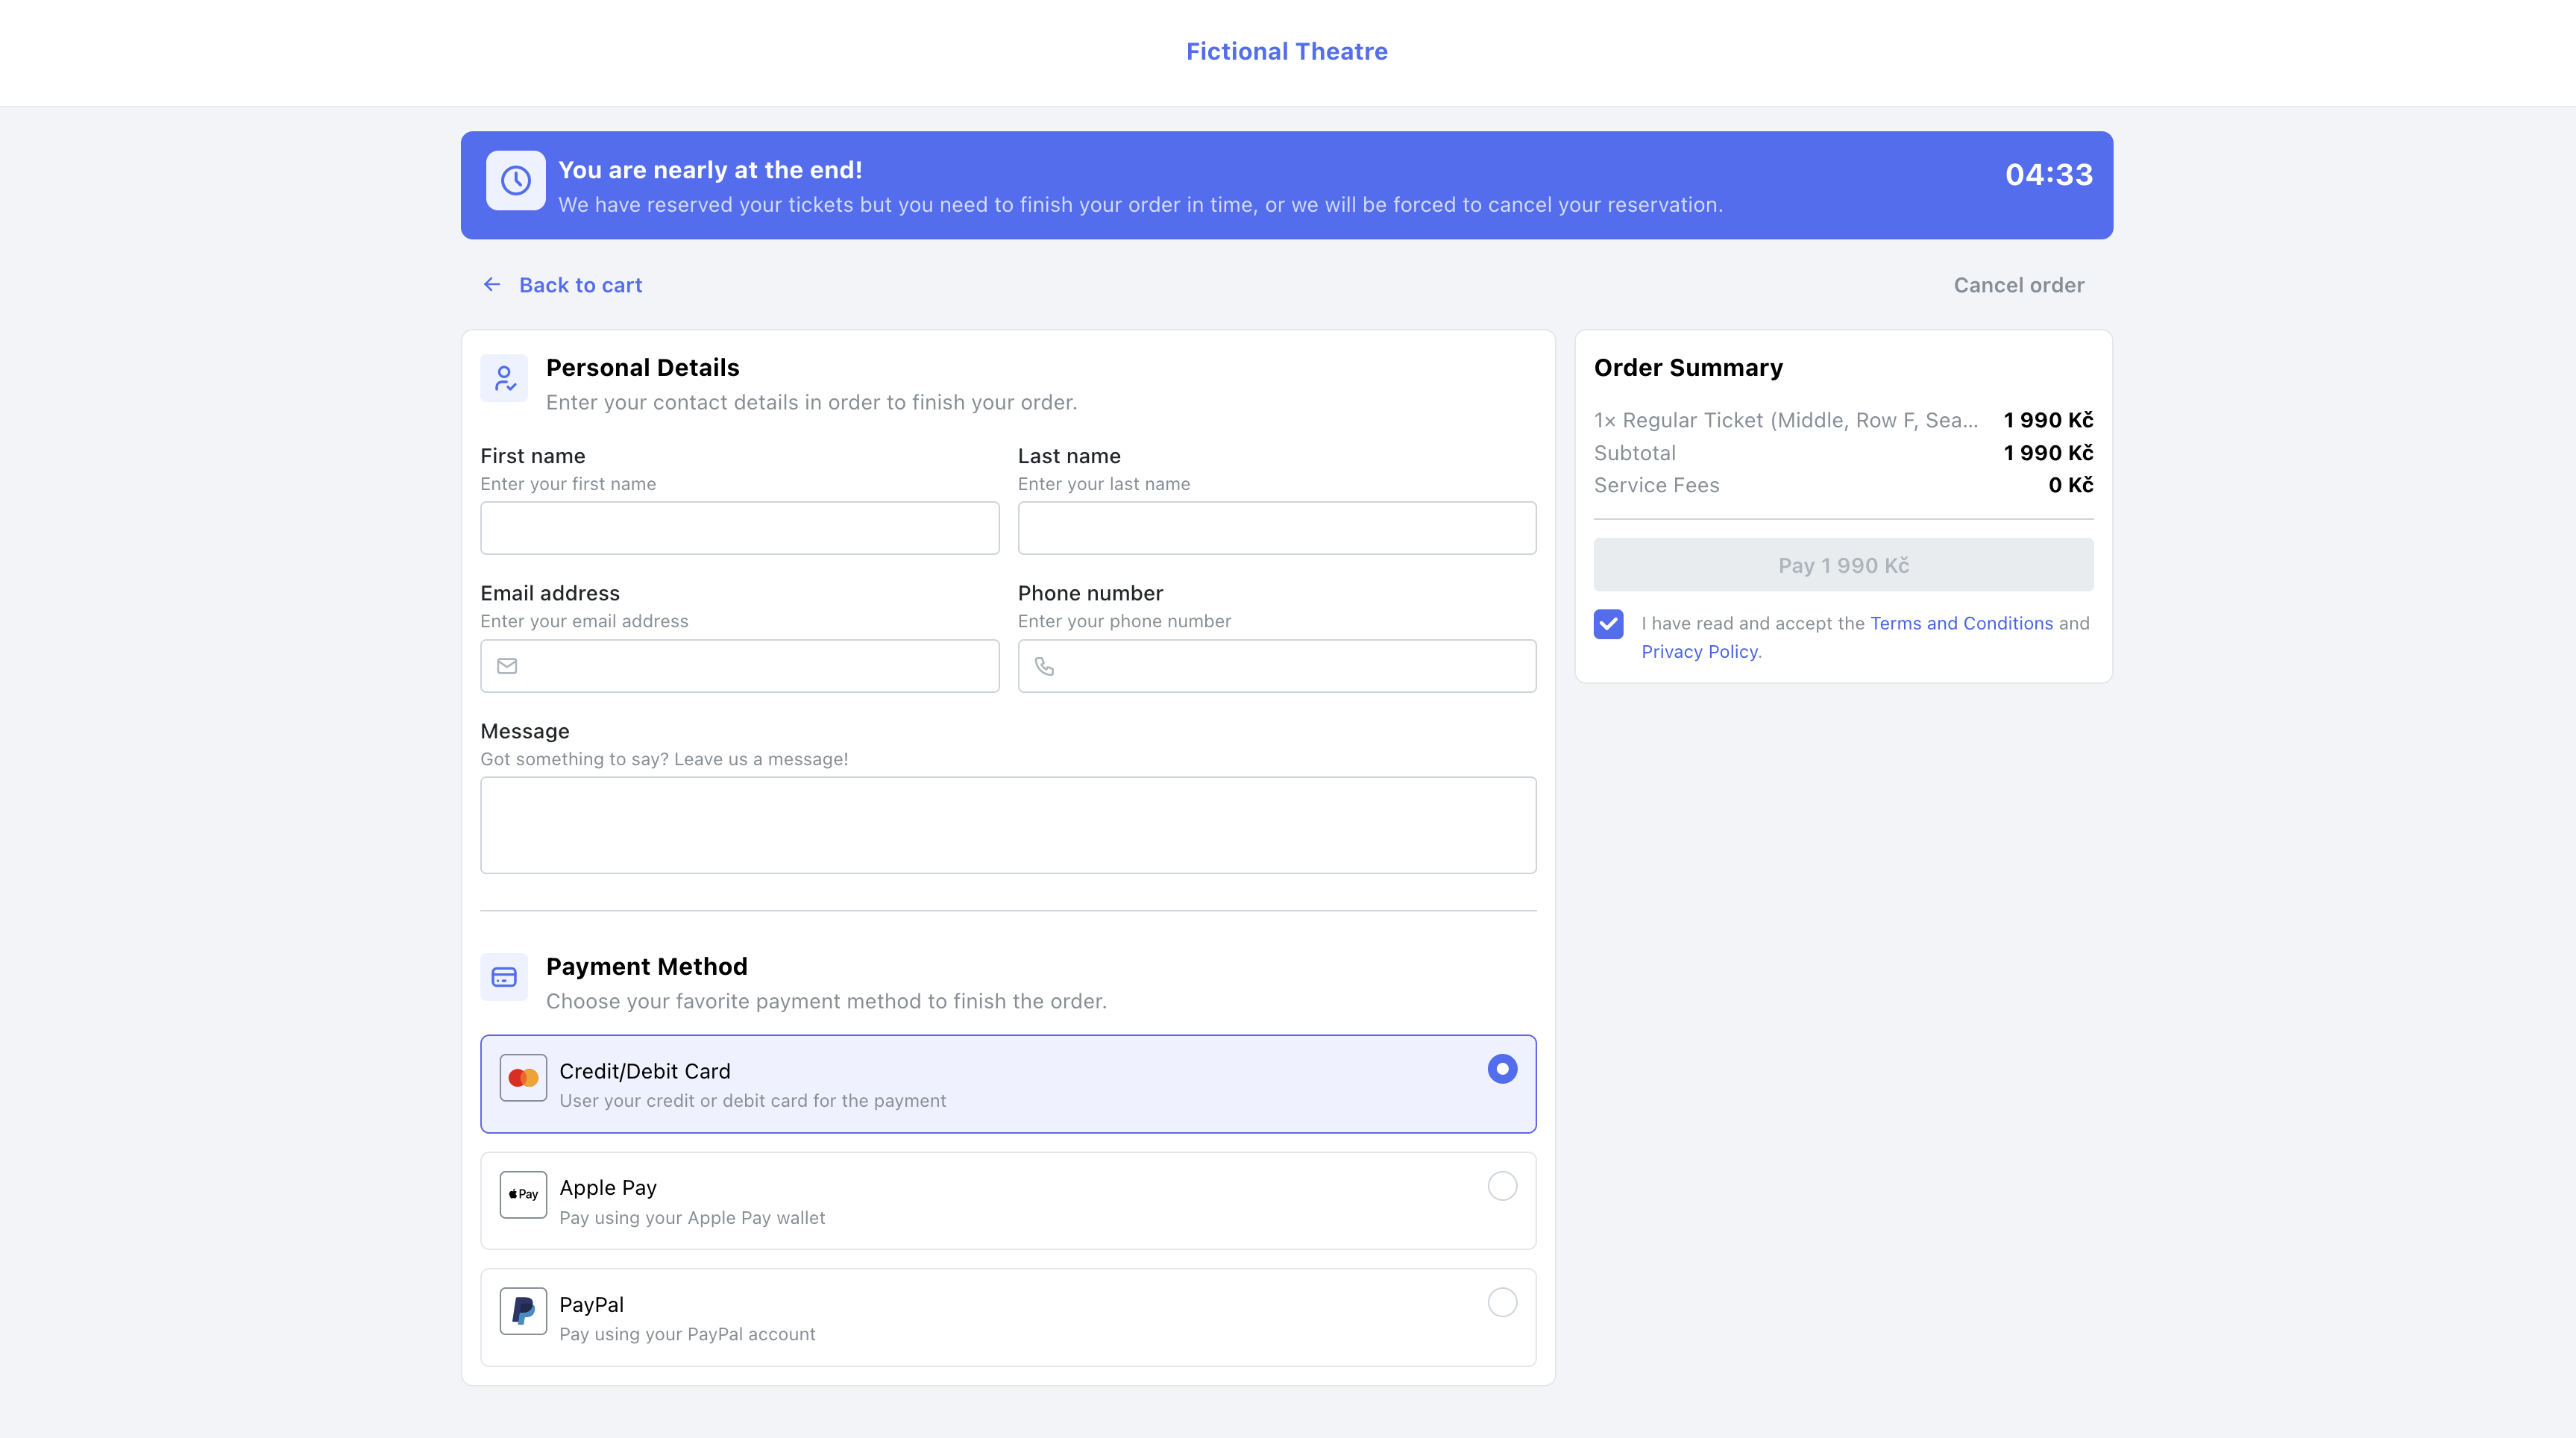
\includegraphics[width=\textwidth]{\FIGDIR/seating-map-checkout}
        \caption{Potvrzení objednávky}
        \label{fig:seating-map-checkout}
    \end{figure}
\end{subsection}

%%% Podsekce – Potvrzení objednávky
%%%%% Wording: ✅
%%%%% Styling: ✅
%%%%% References: ✅
%%% --------------------------------------------------------------
\begin{subsection}{Potvrzení objednávky}
    \label{subsec:implementace-checkout-order-confirmation}
    Jako poslední krok procesu nákupu vstupenek je implementována stránka s potvrzením objednávky.
    I když je tato stránka úzce propojena s procesem platby, který není součástí této práce, je implementována alespoň velmi jednoduše.

    Jak je navrženo v návrhu uživatelského rozhraní, stránka s potvrzením objednávky obsahuje jednoduchou kartu s jejím přehledem a možností stáhnout si vstupenky.
    V rámci metody \texttt{createOrderHandler()} je vytvořena nová objednávka, která je následně zobrazena na této stránce přístupem k výsledku volání handleru \texttt{createOrderHandler}.

    \begin{figure}[H]
        \centering
        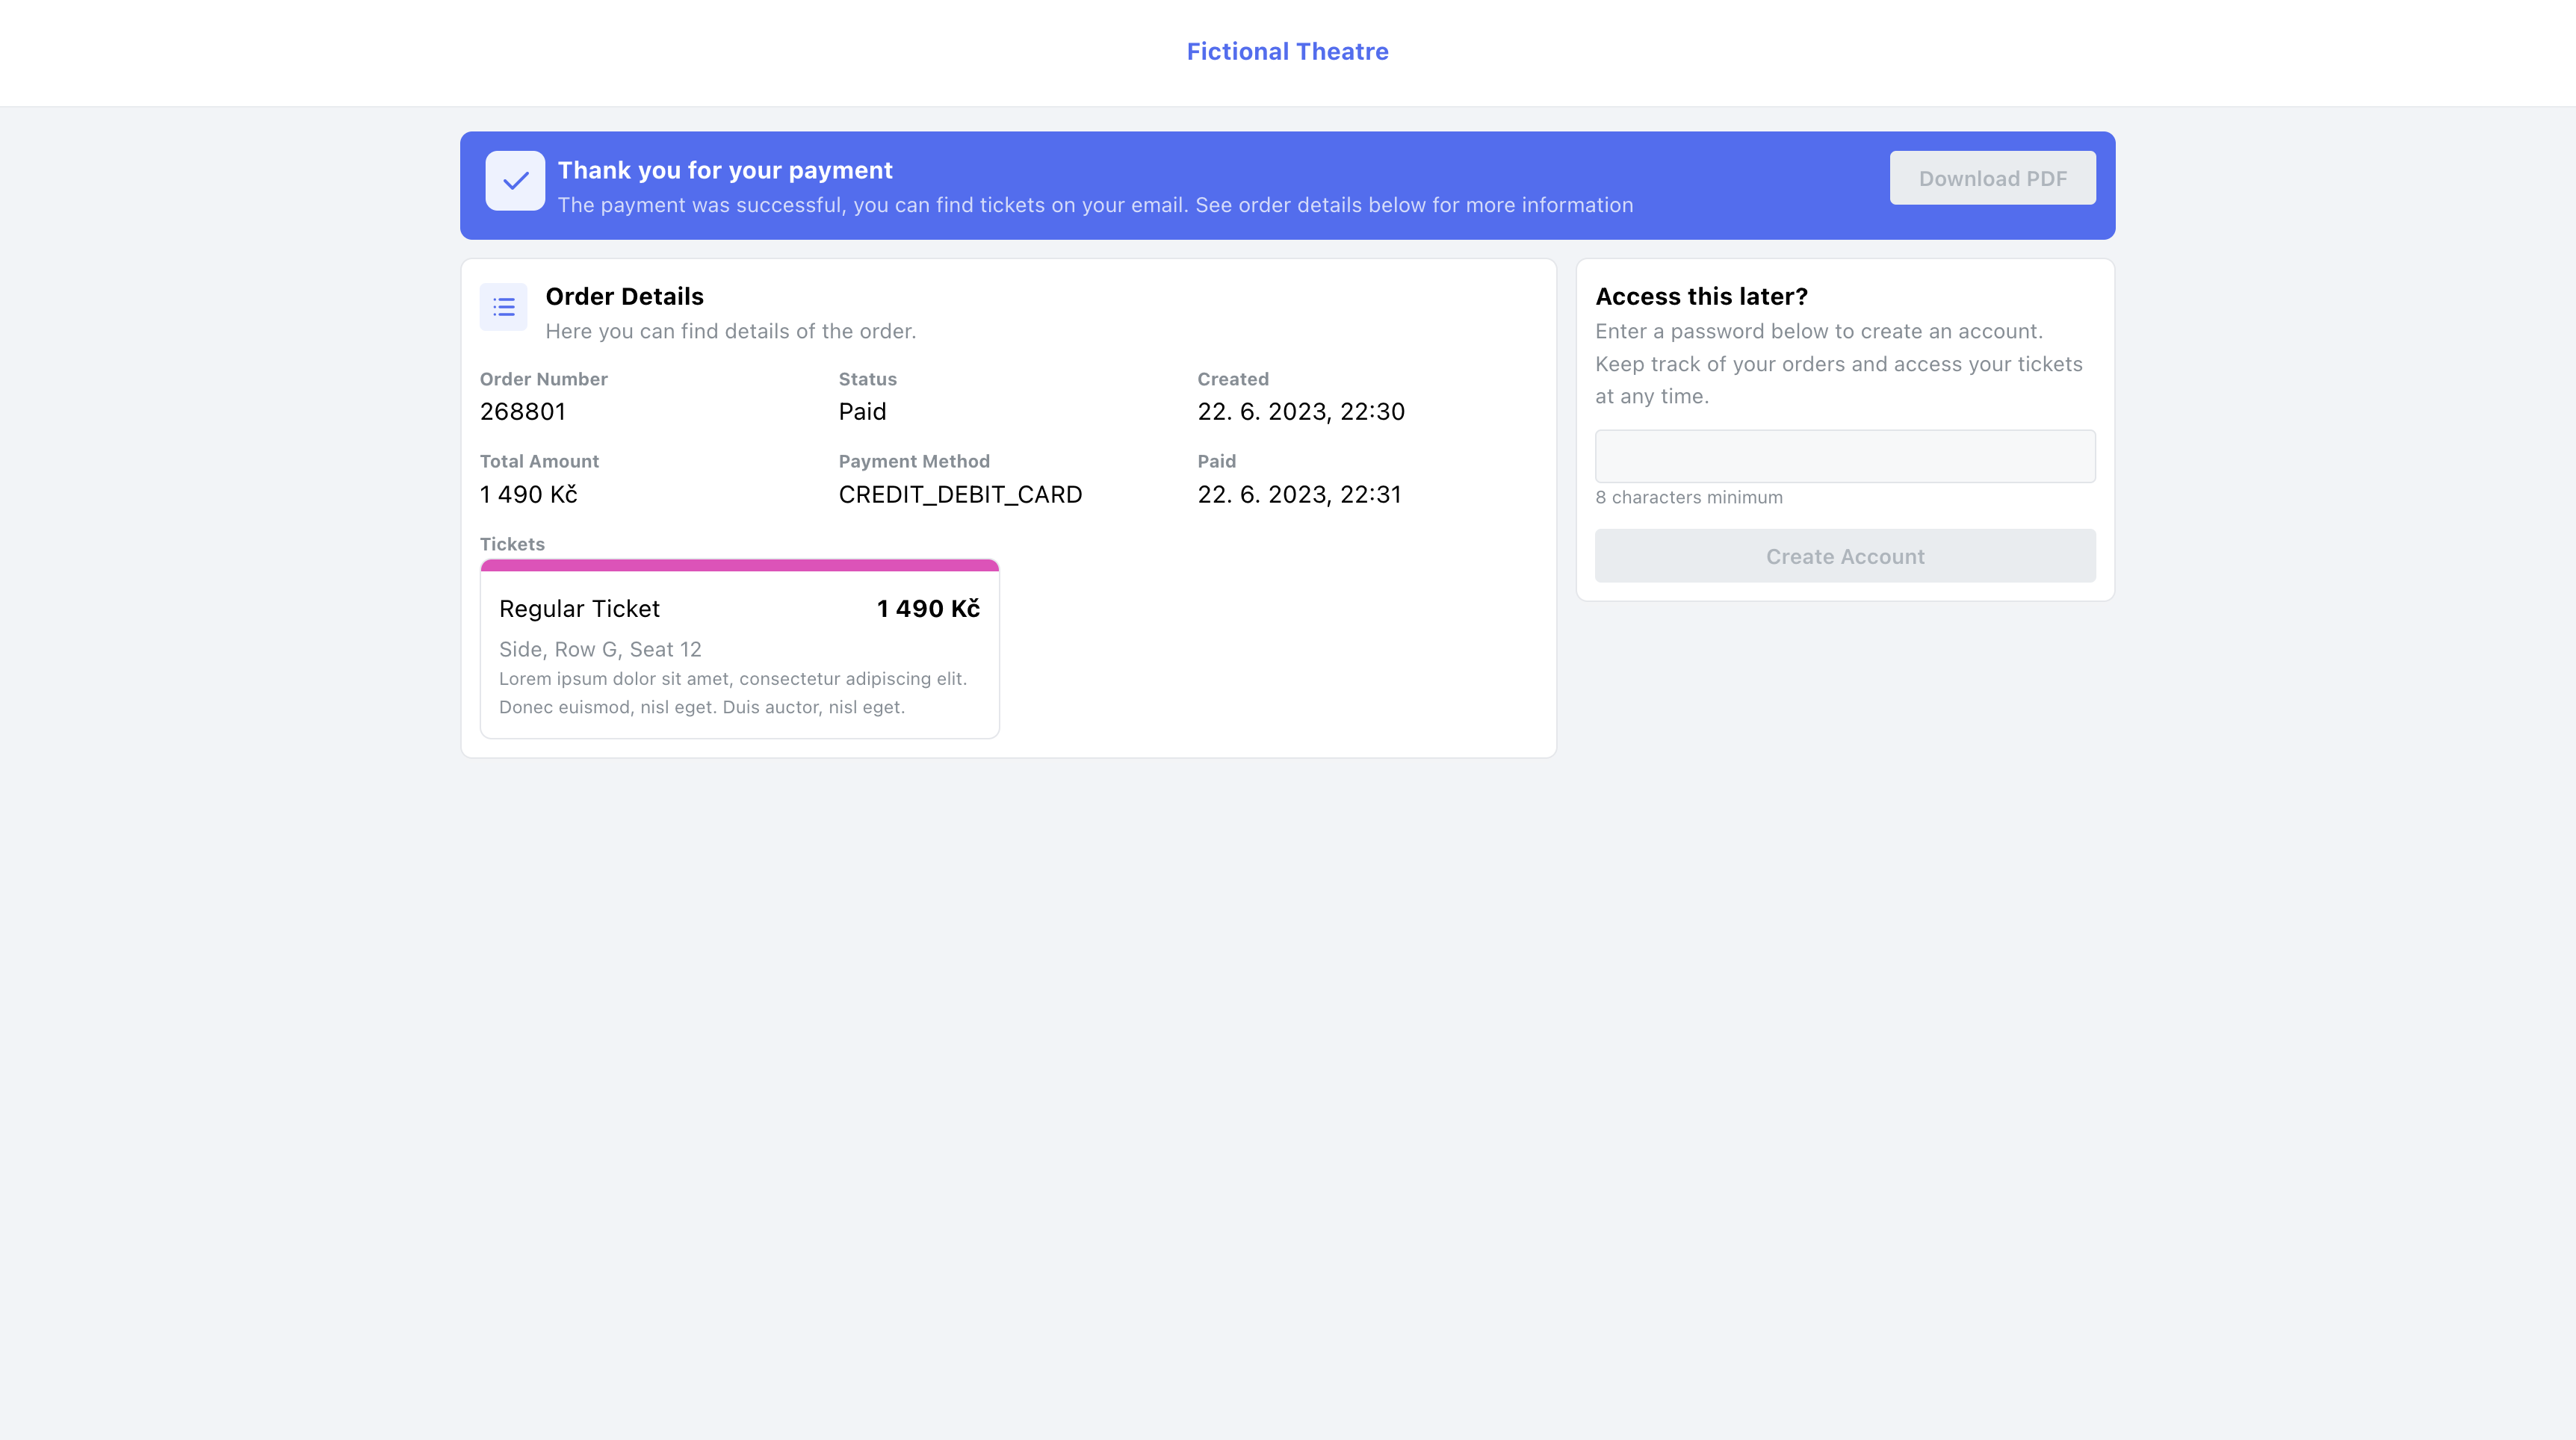
\includegraphics[width=\textwidth]{\FIGDIR/seating-map-order}
        \caption{Stránka s potvrzením objednávky}
        \label{fig:seating-map-order}
    \end{figure}

    Tato finální stránka, zobrazena na obrázku~\ref{fig:seating-map-order}, je také posledním krokem implementační části vyvíjené aplikace.
\end{subsection}
